\section{Algorithm Description}\label{sec:algo}

Description of the algorithm and geometric arguments with some explanatory figures. Fig.~\ref{fig:roomshape_algo} illustrates the algorithm used in room shape detection.

\begin{figure}[h!t]
\center{
\fbox{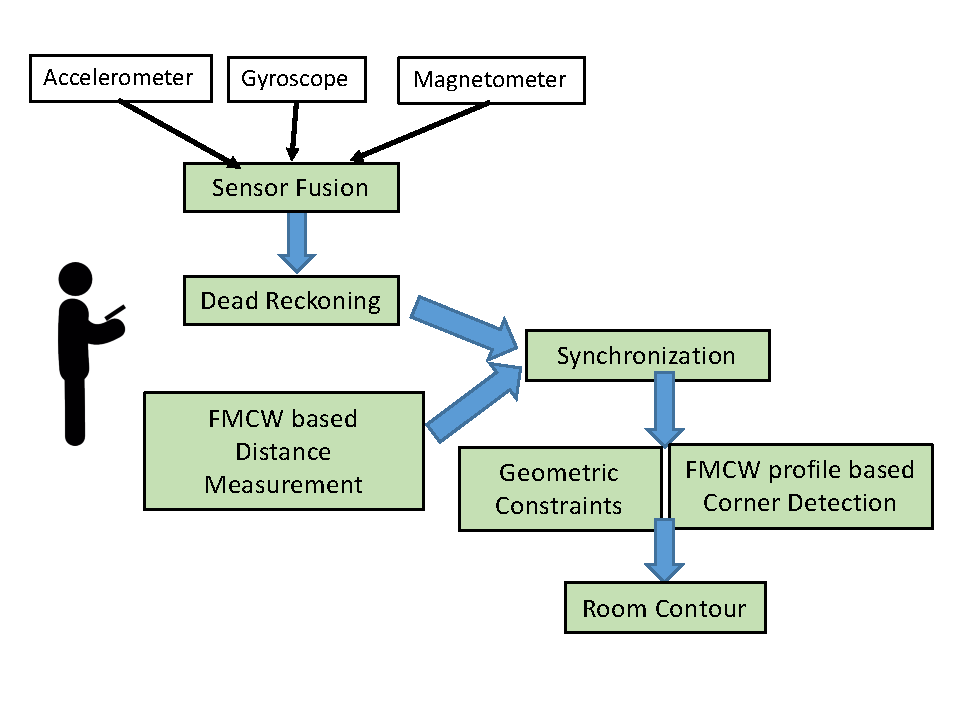
\includegraphics[width=\columnwidth]{figs/roomshape_algo.pdf}}
\caption{Algorithm sketch of \textit{Batphone}}
\label{fig:roomshape_algo}
}
\end{figure}

\begin{algorithm}
    %\vspace{-12pt}
    \caption{\singletag}\label{alg:batphone}
    \begin{algorithmic}[1] 
        \State $x_0 \gets $ current phone orientation 
        \State $p(x) \gets $ current position of the person

        \Procedure{Step Detection}{$\mathbf{a}$}
         		\If{$Acc > Th$}
                    \textbf{return} \texttt{True}
                \EndIf
            \State \textbf{return} \texttt{False}
        \EndProcedure

        \Procedure{getDeadReckoning}{}
            \State $t_0 \gets $ \textsc{currentSystemTime} 
            \State $t \gets t_0$
            \State $\mathbf{w} \gets $ \textsc{emptyVector}
%            \While{$t \leq t_0 + T$}
%                \State $t \gets $ \textsc{currentSystemTime}
%                \State $\mathbf{w} \gets $ \textsc{append}($\mathbf{w}$,
%                    \textsc{currentPhaseReading})
%            \EndWhile
            \State \textbf{return} \texttt{True}
        \EndProcedure

        \Procedure{updateLocation}{$x_0, \mathbf{w}$}
            \State $x_\mathrm{new} \gets \argmin_{x_\mathrm{min} < x <
                x_\mathrm{max}} $ \Call{minDTW}{$x_0, x, \mathbf{w}$}
            \State \textbf{return} $x_\mathrm{new}$
        \EndProcedure

%        \Procedure{touchDetection}{}
%            \While{\texttt{True}}
%                \State $\mathbf{w} \gets $\Call{getPhaseData}{} 
%                \If{$\mathbf{mean}(\mathbf{w}) > C$}
%                    \textbf{return} \texttt{True}
%                \EndIf
%            \EndWhile
%        \EndProcedure
%
%        \Procedure{touchTracking}{}
%            \While{\texttt{True}} 
%                \State $\mathbf{w} \gets $\Call{getPhaseData}{} 
%                \State $x_0 \gets $ \Call{updateLocation}{$x_0, \mathbf{w}$}
%            \EndWhile
%        \EndProcedure
%
%        \State \textsc{touchDetection}();
%        \State \textsc{touchTracking}();
    \end{algorithmic}
    %\vspace{-12pt}
\end{algorithm}